%% 使用 njuthesis 文档类生成南京大学学位论文的示例文档
%%
%% 作者:梁宇钦,YusnowsLiang(at) gmail (dot) com
%% 项目主页: https://github.com/Yusnows/nju-thesis
%%
\documentclass[12pt,a4paper]{article}

\usepackage[utf8]{inputenc}
\usepackage{array}
\usepackage{multirow}
\usepackage{amsmath}
\usepackage{amsfonts}
\usepackage{amssymb}
\usepackage{makeidx}
 \usepackage[a4paper,top=2cm,bottom=2cm,left=2cm,right=2cm]{geometry} % 页边距

%%% 字体设置


%\setmainfont{Times New Roman}
%\setsansfont{Myriad Pro}
%\setmonofont{Courier Std}



%标题与正文间距设置
 
\usepackage{booktabs}%表格
\renewcommand{\tablename}{表}
\usepackage{longtable}

%目录设置
 \usepackage{titletoc}
 \titlecontents{section}[0pt]{\addvspace{4mm}\filright}
 {\bfseries\contentspush{\bfseries{\thecontentslabel}\hspace{1.2mm}\ }}
 {}{\titlerule*[3pt]{\bf{.}}\hspace*{-0.8em}\bf{\contentspage}}
\usepackage[bookmarks=true,colorlinks,linkcolor=black]{hyperref}
\renewcommand{\contentsname}{目录}

\usepackage{abstract}
\renewcommand{\abstractname}{}

\usepackage{cite}
\renewcommand{\refname}{参考文献}

\usepackage{graphicx} %图片
\renewcommand{\figurename}{图}

\usepackage{xeCJK}  %中文支持

%首行缩进以及行间距
%\usepackage{indentfirst}
\usepackage{setspace}

\usepackage{xcolor}
\usepackage{url}

%代码
\usepackage{listings}
\lstset{
  language=python,
  basicstyle=\small,
  numbers=left,
  keywordstyle=\color{blue},
  numberstyle={\normal\color{gray}},
  stepnumber=1, %行号会逐行往上递增
  numbersep=5pt,
  commentstyle=\small\color{green},
  backgroundcolor=\color[rgb]{1.0,1.0,1.0},
  showspaces=false,
  showtabs=false,
  frame=shadowbox, 
  framexleftmargin=5mm, rulesepcolor=\color{red!20!green!20!blue!20!},
  %frame=single,
  %TABframe=single,
  tabsize=2,
  breaklines=tr,
  extendedchars=false, %这一条命令可以解决代码跨页时,章节标题,页眉等汉字不显示的问题
  xleftmargin=3em,
  %	xrightmargin=2em,
  aboveskip=1em,
  escapeinside=``
}


%正文模式
\newcommand{\normal}{	
	\normalsize       
	\setstretch{1.25}		%1.25倍行距
	\setlength{\parindent}{2em}	%首行缩进2字符
	\addtolength{\parskip}{5pt}	%段后空出5pt
}

\newcommand{\titleen}{
  \setstretch{1.1}		%1.25倍行距
  \setlength{\parindent}{0em}	%首行缩进2字符
  \addtolength{\parskip}{1pt}	%段后空出5pt
}

%长度固定的下划线
\makeatletter
\newcommand\dlmu[2][4cm]{\hskip1pt\underline{\hb@xt@ #1{\hss#2\hss}}\hskip3pt}
\makeatother
%%%%%%%%%%%%%%

\newcommand{\tabincell}[2]{\begin{tabular}{@{}#1@{}}#2\end{tabular}}  %表格自动换行

\newcommand{\tpar}{
	\normalsize
	\setstretch{1.25}		%1.25倍行距
	\hspace{1.5em}
}

\newcommand{\epar}{
	\vspace{3pt}
}
\RequirePackage{fontspec}
\setCJKmainfont[BoldFont={Microsoft YaHei}, ItalicFont={Microsoft YaHei}, BoldItalicFont={Microsoft YaHei}]{Adobe Song Std}
\setCJKsansfont{Microsoft YaHei}
\setCJKmonofont{Microsoft YaHei}

\title{\textbf{南京大学本科毕业论文(设计)开题报告}}
\date{}

\begin{document}
	
	\maketitle
	\vspace{-20mm}
	\centering
	\small
	填表人姓名: \dlmu[2cm]{} \hspace{5mm}填表时间:\dlmu[1cm]{}年\dlmu[1cm]{}月\dlmu[1cm]{}日
	\vspace{-4mm}
	\setstretch{1.5}
	\normalsize
	\begin{longtable}{|>{\centering\arraybackslash}p{3cm}|>{\centering\arraybackslash}p{5cm}|>{\centering\arraybackslash}p{2cm}|>{\centering\arraybackslash}p{3.5cm}|}
		%长表格的连接处设置,不用管
		\hline
		\endhead
		\endfirsthead
		\hline
		\endfoot
		\endlastfoot
		
		%下面是表头的设置
		\hline 
		学生姓名 & 梁宇钦 &  学号 & 151180076 \\ 
		\hline 
 		院系专业 & 电子信息科学技术 & 手机号 & 159******** \\ 
		\hline 
 		指导老师姓名 & 雷军 & 职称 & 教授 \\ 
		\hline 
		所在院系/单位 & \multicolumn{3}{c|}{$\blacksquare$ 校内:\dlmu[3.5cm]{\small 电子科学与工程学院 \normalsize} \hspace{10mm} $\Box$校外: \dlmu[3cm]{}}  \\ 
		\hline 
		论文题目 & \multicolumn{3}{c|}{王母娘娘寿筵上蟠桃生长过程仿真与分析} \\ 
		\hline 
		%下面开始是正文,正文全都需要把4栏表格合成一栏,因此所有段落的开头都需要使用 \multicolumn{4}{|p{15cm}|}{ 内容在这写 }\\ 命令, 但是由于首段需要缩进,以及段落之间需要隔开一定距离,所以变成了 \multicolumn{4}{|p{15cm}|}{ \tpar 内容在这写 \epar}\\ 或者 \multicolumn{4}{|p{15cm}|}{\texbf{标题}\par \normal 内容在这写 \epar }\\ 这样的。对于一些可能一段内容在一页放不下的情况,需要手动用 \multicolumn{4}{|p{15cm}|}{ 内容在这写 }\\ 进行分割
		\multicolumn{4}{|p{15cm}|}{
			\textbf{一、研究背景及意义}(附参考文献,不少于800字)\par  
			\normal
			文献\cite{scoliosis-baidu};中提到:一朝,王母娘娘设宴,大开宝阁,瑶池中做“蟠桃胜会”,
			即着那红衣仙女、素衣仙女、青衣仙女、皂衣仙女、紫衣仙女、黄衣仙女、绿衣仙女\cite{Liu2009},各顶花篮,去蟠桃园摘桃建会。七衣仙女直至园门首,只见蟠桃园土地、力士同齐天府二司仙吏,都在那里把门。仙女近前道:“我等奉王母懿旨,到此携桃设宴。”土地道:“仙娥且住。今岁不比往年了,玉帝点差齐天大圣在此督理,须是报大圣得知,方敢开园。”仙女道:“大圣何在?”土地道:“大圣在园内,因困倦,自家在亭子上睡哩。”仙女道:“。既如此,寻他去来,不可延误。”\cite{scoliosis-baidu}。土地即与同进。寻至花亭不见,只有衣冠在亭,不知何往。四下里都没寻处。原来大圣耍了一会,吃了几个桃子,变做二寸长的个人儿,在那大树梢头浓叶之下睡着了。七衣仙女道:“我等奉旨前来,寻不见大圣,怎敢空回?”旁有仙吏道:“仙娥既奉旨来,不必迟疑。我大圣闲游惯了,想是出园会友去了。汝等且去摘桃,我们替你回话便是。\cite{Liu2009,Drerup2014}”那仙女依言,入树林之下摘桃。先在前树摘了二篮,又在中树摘了三篮;到后树上摘取,只见那树上花果稀疏,止有几个毛蒂青皮的。原来熟的都是猴王吃了。七仙女张望东西\cite{StevenS2008},只见南枝上止有一个半红半白的桃子。青衣女用手扯下枝来,红衣女摘了,却将枝子望上一放。原来那大圣变化了,正睡在此枝,被他惊醒。大圣即现本相,耳朵内掣出金箍棒\cite{RoweDE1997},幌一幌,碗来粗细,咄的一声道:“你是那方怪物,敢大胆偷摘我桃!”慌得那七仙女一齐跪下道:“大圣息怒。我等不是妖怪,乃王母娘娘差来的七衣仙女,摘取仙桃,大开宝阁,做‘蟠桃胜会’。适至此间,先见了本园土地等神,寻大圣不见。我等恐迟了王母懿旨,是以等不得大圣,故先在此摘桃,万望恕罪。”大圣闻言,回嗔作喜道:“仙娥请起。王母开阁设宴,请的是谁?”仙女道:“上会自有旧规。请的是西天佛老、菩萨、罗汉,南方南极观音,东方崇恩圣帝,十洲三岛仙翁\cite{Nachemson1995},北方北极玄灵,中央黄极黄角大仙,这个是五方五老。还有五斗星君,上八洞三清、四帝、太乙天仙等众,中八洞玉皇、九垒、海岳神仙,下八洞幽冥教主、注世地仙。各宫各殿大小尊神,俱一齐赴蟠桃嘉会。”大圣笑道:“可请我么?”仙女说:“不曾听得说。”大圣道:“我乃齐天大圣\cite{Knott2014},就请我老孙做个尊席,有何不可?”仙女道:“此是上会会规,今会不知如何。”大圣道:“此言也是,难怪汝等。你且立下,待老孙先去打听个消息,\epar }\\
		
		\multicolumn{4}{|p{15cm}|}{
			看可请老孙不请。”好大圣,捻着诀,念声咒语,对众仙女道:“住!住!住!”这原来是个定身法,把那七衣仙女一个个睖睖睁睁,白着眼,都站在桃树之下。大圣纵朵祥云,跳出园内,竟奔瑶池路\cite{Patias2010}上而去\epar }\\
		
		\multicolumn{4}{|p{15cm}|}{\tpar
			名称赤脚大罗仙,特赴蟠桃添寿节。那赤脚大仙觌面撞见大圣,大圣低头定计,赚哄真仙,他要暗去赴会,却问:“老道何往?”大仙道:“蒙王母见招,去赴蟠桃嘉会。”大圣道:“老道不知。玉帝因老孙筋斗云疾,着老孙五路邀请列位,先至通明殿下演礼,后方去赴宴。\cite{Spinal2008,Knott2014,PhysRehabil2012}”大仙是个光明正大之人,就以他的诳语作真。道:“常年就在瑶池演礼谢恩,如何先去通明殿演礼,方去瑶池赴会?”无奈,只得拨转祥云,径往通明殿去了。\epar }\\
		
		\multicolumn{4}{|p{15cm}|}{\tpar
			 大圣驾着云,念声咒语,摇身一变,就变做赤脚大仙模样,前奔瑶池。不多时,直至宝阁,按住云头,轻轻移步,走入里面。只见那里:琼香缭绕,瑞霭缤纷\cite{Liu2009},瑶台铺彩结,宝阁散氤氲。凤翥鸾腾形缥缈,金花玉萼影浮沉。上排着九凤丹霞扆,八宝紫霓墩。五彩描金桌,千花碧玉盆。桌上有龙肝和凤髓,熊掌与猩唇\cite{Drerup2014}。珍馐百味般般美,异果嘉肴色色新。\epar}\\
		\hline
		\multicolumn{4}{|p{15cm}|}{
			\textbf{二、国内外研究现状}(文献综述,附参考文献,不少于1000字)\par  
			\normal
			猴~~哥~~($xxx-$),男,江苏花果山人\cite{Dubousset1992,Perdriolle1987MorphologyOS},法号行者,是唐僧的大徒弟,会七十二变、腾云驾雾。
			一双火眼金睛,能看穿妖魔鬼怪伪装的伎俩;一个筋斗能翻十万八千里;使用的兵器如意金箍棒,能大能小,随心变化,小到绣花针,大到顶天立地。他占花果山为王,自称齐天大圣,搅乱王母娘娘的蟠桃胜会,偷吃太上老君的长生不老金丹,打败天宫十万天兵天将\cite{Drerup2014},又自不量力地与如来佛祖斗法,被压在五行山下五百多年。后来经观世音菩萨点化,保护唐僧西天取经,三打白骨精,收服红孩儿,熄灭火焰山,一路上降魔斗妖,历经九九八十一难,取回真经终成正果。他嫉恶如仇,不怕困难,坚韧不拔,英勇无畏,取经后被封为斗战胜佛\cite{Liu2009,Mitulescu2001,DUMAS2003827,Mitton2000,ANDRE19941023,Trochu1993,POMERO2004240}。
			\epar } \\
		
		\multicolumn{4}{|p{15cm}|}{\tpar
			 八~~戒~~($xxx-$),男,天宫人,法号悟能,是唐僧的二徒弟,原来是玉皇大帝的天蓬元帅,因调戏嫦娥被逐出天界,到人间投胎,却又错投猪胎,嘴脸与猪相似。他会变身术,能腾云驾雾,使用的兵器是九齿钉钯。唐僧西去取经路过云栈洞,猪八戒被孙悟空收服,八戒从此成为孙悟空的好帮手,一同保护唐僧西天取经。八戒性格温和,憨厚单纯\cite{Liu2009,Mitulescu2001,DUMAS2003827,Mitton2000,ANDRE19941023,Trochu1993,POMERO2004240},力气大,但又好吃懒做,爱占小便宜,贪图女色,经常被妖怪的美色所迷,难分敌我。他对师兄的话言听计从,对师父忠心耿耿,为唐僧西天取经立下汗马功劳,是个被人们喜爱同情的喜剧人物。
			\epar}\\
		
		\multicolumn{4}{|p{15cm}|}{
			\textbf{2.1 猴王大闹天宫}\par
			\normal
			文献\cite{scoliosis-baidu};中提到:一朝,王母娘娘设宴,大开宝阁,瑶池中做“蟠桃胜会”,
			即着那红衣仙女、素衣仙女、青衣仙女、皂衣仙女、紫衣仙女、黄衣仙女、绿衣仙女\cite{Mitton2000},各顶花篮,去蟠桃园摘桃建会。七衣仙女直至园门首,只见蟠桃园土地、
		\epar}\\
	
		\multicolumn{4}{|p{15cm}|}{
			力士同齐天府二司仙吏,都在那里把门。仙女近前道:“我等奉王母懿旨,到此携桃设宴。”土地道:“仙娥且住。今岁不比往年了,玉帝点差齐天大圣在此督理,须是报大圣得知,方敢开园。”仙女道:“大圣何在?”土地道:“大圣在园内,因困倦,自家在亭子上睡哩。”仙女道:“。既如此,寻他去来,不可延误。”\cite{Trochu1993}。土地即与同进。寻至花亭不见,只有衣冠在亭,不知何往。四下里都没寻处。原来大圣耍了一会,吃了几个桃子,变做二寸长的个人儿,在那大树梢头浓叶之下睡着了。
			\epar}\\
		
		\multicolumn{4}{|p{15cm}|}{\tpar
			七衣仙女道:“我等奉旨前来,寻不见大圣,怎敢空回?”旁有仙吏道:“仙娥既奉旨来,不必迟疑。我大圣闲游惯了,想是出园会友去了。汝等且去摘桃,我们替你回话便是\cite{Perdriolle1987MorphologyOS}”那仙女依言,入树林之下摘桃。先在前树摘了二篮,又在中树摘了三篮;到后树上摘取,只见那树上花果稀疏,止有几个毛蒂青皮的。原来熟的都是猴王吃了。
		\epar}\\
		
		\multicolumn{4}{|p{15cm}|}{
			\textbf{2.2 猪八戒调戏嫦娥}\par
			\normal
			\begin{equation}
				a = b
				\label{e1}
			\end{equation}
%			\begin{figure}
%				\centering
%				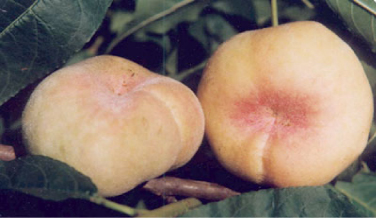
\includegraphics[width=12cm]{figures/Pantao}
%			\end{figure}
			七仙女张望东西\cite{Drerup2014},只见南枝上止有一个半红半白的桃子。青衣女用手扯下枝来,红衣女摘了,却将枝子望上一放。原来那大圣变化了,正睡在此枝,被他惊醒。大圣即现本相,耳朵内掣出金箍棒\cite{RoweDE1997},幌一幌,碗来粗细,咄的一声道:“你是那方怪物,敢大胆偷摘我桃!”慌得那七仙女一齐跪下道:“大圣息怒。我等不是妖怪,乃王母娘娘差来的七衣仙女,摘取仙桃,大开宝阁,做‘蟠桃胜会\ref{e1}’。适至此间,先见了本园土地等神,寻大圣不见。我等恐迟了王母懿旨,是以等不得大圣,故先在此摘桃,万望恕罪。”大圣闻言,回嗔作喜道:“仙娥请起。王母开阁设宴,请的是谁?”仙女道:“上会自有旧规。请的是西天佛老、菩萨、罗汉,南方南极观音,东方崇恩圣帝,十洲三岛仙翁\cite{optimized-boyd},北方北极玄灵,中央黄极黄角大仙,这个是五方五老。还有五斗星君,上八洞三清、四帝、太乙天仙等众,中八洞玉皇、九垒、海岳神仙,下八洞幽冥教主、注世地仙。各宫各殿大小尊神,俱一齐赴蟠桃嘉会。”大圣笑道:“可请我么?”仙女说:“不曾听得说。”大圣道:“我乃齐天大圣\cite{cobb-wiki},就请我老孙做个尊席,有何不可?”仙女道:“此是上会会规,今会不知如何。”大圣道:“此言也是,难怪汝等。你且立下,待老孙先去打听个消息,看可请老孙不请。”好大圣,捻着诀,念声咒语,对众仙女道:“住!住!住!”这原来是个定身法,把那七衣仙女一个个睖睖睁睁,白着眼,都站在桃树之下。大圣纵朵祥云,跳出园内,竟奔瑶池路。\epar} \\
		
		\hline 
		\multicolumn{4}{|p{15cm}|}{
			\textbf{三、主要研究或解决的问题和拟采用的方法} \par 
			\vspace{3mm}
			\textbf{3.1 研究目的} \par
			\normal 
			蟠桃真好吃,当时真是吃少了,现在需要研究研究,希望能给花果山的孩儿们栽上几棵,尝尝鲜。
		\epar }\\ 
	
		\multicolumn{4}{|p{15cm}|}{
			\textbf{3.2 研究内容} \par 
			\normal
			基于以上研究目的,本研究拟从以下几个方面展开研究。
			\begin{enumerate}
			\setstretch{1.0}
			\item 首先培育众多仙女。
			\item 让培育好的仙女种植很多的蟠桃树。
			\item 建立蟠桃树成长过程的仿真系统,根据仿真结果制定照料方案。让仙女们严格按照仿真指导工作。
			\item 争取一年就让蟠桃树从树苗长成参天大树,并结出果实。
			\end{enumerate}
		} \\ 
	
		\multicolumn{4}{|p{15cm}|}{
			\textbf{3.3 研究方法和路径} \par 
			\normal
			\begin{minipage}[t]{14cm}
				\centering
				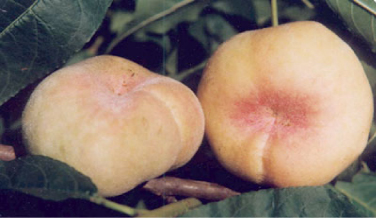
\includegraphics[width=12cm]{figures/Pantao}
			\end{minipage}
		} \\ 
		\multicolumn{4}{|p{15cm}|}{
			\centering \small 图1. 研究方法和研究路径
		\epar} \\
	
		\multicolumn{4}{|p{15cm}|}{	\tpar
			如图1所示,首先培育众多仙女。 让培育好的仙女种植很多的蟠桃树。建立蟠桃树成长过程的仿真系统,根据仿真结果制定照料方案。让仙女们严格按照仿真指导工作。争取一年就让蟠桃树从树苗长成参天大树,并结出果实。
		\epar} \\
		
		\hline 
		\multicolumn{4}{|p{15cm}|}{
			\textbf{四、工作进度计划}(每两周为一个单位)\par  
			\normal
			\begin{itemize}
				\item 1-2周:查阅相关文献资料,获取培育众多仙女方法。
				\item 3-4周:进行培育众多仙女的实验。
				\item 5-6周:查阅相关文献资料,获取脊让培育好的仙女种植很多的蟠桃树的方案。
				\item 7-8周:让培育好的仙女种植很多的蟠桃树。
				\item 9-10周:建立蟠桃树成长过程的仿真系统。
			\end{itemize}
		} \\ 
	 
		\multicolumn{4}{|p{15cm}|}{
			\vspace{-10mm}
			\begin{itemize}
				\item 11-12周:进行仿真实验,根据仿真结果制定照料方案。让仙女们严格按照仿真指导工作。
				\item 13-14周:根据实际情况,做一些微调,争取一年就让蟠桃树从树苗长成参天大树,并结出果实。
			\end{itemize}
		} \\
		\hline 
		\multicolumn{4}{|p{15cm}|}{
			\textbf{指导教师意见}(不少于50个字) \par 
			\normal 
			蟠桃真的很好吃,我吹爆。该同学提出的培养蟠桃的方案十分有价值,若是成功,我可以吃蟠桃当作三餐了,我吹爆。该课题选题思路合理,具有一定的研究基础,预期效果良好,同意开题。
			\vspace{20mm}
			\flushright{签名: \dlmu[4cm]{}}
			\flushright{\hspace{3cm}年\hspace{1cm}月\hspace{1cm}日}
			\epar
		} \\  
	\hline 
	\multicolumn{4}{|p{15cm}|}{
		\textbf{院系意见:}  
		\vspace{100pt}
		\flushright{院系负责人签名: \dlmu[4cm]{}}
		\flushright{\hspace{3cm}年\hspace{1cm}月\hspace{1cm}日}
		\epar
	} \\  
	\hline
	\end{longtable}
	\vspace{-5mm}
	% \usepackage{array} is required
	\begin{tabular}{>{\raggedright\arraybackslash}p{15cm}}
		\small
		\setstretch{1.1}
		注:表格栏高不够可自行增加。此表在学生做完开题报告后,上交所在院系留存。待毕业论文完成后按《南京大学本科生毕业论文收集、整理、存档实施细则》进行装订、存档,由院系负责保存。\\ 
	\end{tabular} 


	\newpage
%	\bibliographystyle{IEEEtran}
	\bibliographystyle{gbt7714-2005}
%	\bibliographystyle{elsarticle-num}
	\bibliography{ref/citation.bib}
\end{document}
